\documentclass[justified]{tufte-book}

% ams
\usepackage{amssymb,amsmath}

\usepackage{ifxetex,ifluatex}
\usepackage{fixltx2e} % provides \textsubscript
\ifnum 0\ifxetex 1\fi\ifluatex 1\fi=0 % if pdftex
  \usepackage[T1]{fontenc}
  \usepackage[utf8]{inputenc}
\else % if luatex or xelatex
  \makeatletter
  \@ifpackageloaded{fontspec}{}{\usepackage{fontspec}}
  \makeatother
  \defaultfontfeatures{Ligatures=TeX,Scale=MatchLowercase}
  \makeatletter
  \@ifpackageloaded{soul}{
     \renewcommand\allcapsspacing[1]{{\addfontfeature{LetterSpace=15}#1}}
     \renewcommand\smallcapsspacing[1]{{\addfontfeature{LetterSpace=10}#1}}
   }{}
  \makeatother

\fi

% graphix
\usepackage{graphicx}
\setkeys{Gin}{width=\linewidth,totalheight=\textheight,keepaspectratio}

% booktabs
\usepackage{booktabs}

% url
\usepackage{url}

% hyperref
\usepackage{hyperref}

% units.
\usepackage{units}


\setcounter{secnumdepth}{2}

% citations

\newlength{\cslhangindent}
\setlength{\cslhangindent}{1.5em}
% For Pandoc 2.8 to 2.11
\newenvironment{cslreferences}%
  {\setlength{\parindent}{0pt}%
  \everypar{\setlength{\hangindent}{\cslhangindent}}\ignorespaces}%
  {\par}
% For pandoc 2.11+ using new --citeproc
\newlength{\csllabelwidth}
\setlength{\csllabelwidth}{3em}
\newlength{\cslentryspacingunit} % times entry-spacing
\setlength{\cslentryspacingunit}{\parskip}
\newenvironment{CSLReferences}[2] % #1 hanging-ident, #2 entry spacing
 {% don't indent paragraphs
  \setlength{\parindent}{0pt}
  % turn on hanging indent if param 1 is 1
  \ifodd #1
  \let\oldpar\par
  \def\par{\hangindent=\cslhangindent\oldpar}
  \fi
  % set entry spacing
  \setlength{\parskip}{#2\cslentryspacingunit}
 }%
 {}
\usepackage{calc}
\newcommand{\CSLBlock}[1]{#1\hfill\break}
\newcommand{\CSLLeftMargin}[1]{\parbox[t]{\csllabelwidth}{#1}}
\newcommand{\CSLRightInline}[1]{\parbox[t]{\linewidth - \csllabelwidth}{#1}}
\newcommand{\CSLIndent}[1]{\hspace{\cslhangindent}#1}

% pandoc syntax highlighting
\usepackage{color}
\usepackage{fancyvrb}
\newcommand{\VerbBar}{|}
\newcommand{\VERB}{\Verb[commandchars=\\\{\}]}
\DefineVerbatimEnvironment{Highlighting}{Verbatim}{commandchars=\\\{\}}
% Add ',fontsize=\small' for more characters per line
\newenvironment{Shaded}{}{}
\newcommand{\AlertTok}[1]{\textcolor[rgb]{1.00,0.00,0.00}{\textbf{#1}}}
\newcommand{\AnnotationTok}[1]{\textcolor[rgb]{0.38,0.63,0.69}{\textbf{\textit{#1}}}}
\newcommand{\AttributeTok}[1]{\textcolor[rgb]{0.49,0.56,0.16}{#1}}
\newcommand{\BaseNTok}[1]{\textcolor[rgb]{0.25,0.63,0.44}{#1}}
\newcommand{\BuiltInTok}[1]{#1}
\newcommand{\CharTok}[1]{\textcolor[rgb]{0.25,0.44,0.63}{#1}}
\newcommand{\CommentTok}[1]{\textcolor[rgb]{0.38,0.63,0.69}{\textit{#1}}}
\newcommand{\CommentVarTok}[1]{\textcolor[rgb]{0.38,0.63,0.69}{\textbf{\textit{#1}}}}
\newcommand{\ConstantTok}[1]{\textcolor[rgb]{0.53,0.00,0.00}{#1}}
\newcommand{\ControlFlowTok}[1]{\textcolor[rgb]{0.00,0.44,0.13}{\textbf{#1}}}
\newcommand{\DataTypeTok}[1]{\textcolor[rgb]{0.56,0.13,0.00}{#1}}
\newcommand{\DecValTok}[1]{\textcolor[rgb]{0.25,0.63,0.44}{#1}}
\newcommand{\DocumentationTok}[1]{\textcolor[rgb]{0.73,0.13,0.13}{\textit{#1}}}
\newcommand{\ErrorTok}[1]{\textcolor[rgb]{1.00,0.00,0.00}{\textbf{#1}}}
\newcommand{\ExtensionTok}[1]{#1}
\newcommand{\FloatTok}[1]{\textcolor[rgb]{0.25,0.63,0.44}{#1}}
\newcommand{\FunctionTok}[1]{\textcolor[rgb]{0.02,0.16,0.49}{#1}}
\newcommand{\ImportTok}[1]{#1}
\newcommand{\InformationTok}[1]{\textcolor[rgb]{0.38,0.63,0.69}{\textbf{\textit{#1}}}}
\newcommand{\KeywordTok}[1]{\textcolor[rgb]{0.00,0.44,0.13}{\textbf{#1}}}
\newcommand{\NormalTok}[1]{#1}
\newcommand{\OperatorTok}[1]{\textcolor[rgb]{0.40,0.40,0.40}{#1}}
\newcommand{\OtherTok}[1]{\textcolor[rgb]{0.00,0.44,0.13}{#1}}
\newcommand{\PreprocessorTok}[1]{\textcolor[rgb]{0.74,0.48,0.00}{#1}}
\newcommand{\RegionMarkerTok}[1]{#1}
\newcommand{\SpecialCharTok}[1]{\textcolor[rgb]{0.25,0.44,0.63}{#1}}
\newcommand{\SpecialStringTok}[1]{\textcolor[rgb]{0.73,0.40,0.53}{#1}}
\newcommand{\StringTok}[1]{\textcolor[rgb]{0.25,0.44,0.63}{#1}}
\newcommand{\VariableTok}[1]{\textcolor[rgb]{0.10,0.09,0.49}{#1}}
\newcommand{\VerbatimStringTok}[1]{\textcolor[rgb]{0.25,0.44,0.63}{#1}}
\newcommand{\WarningTok}[1]{\textcolor[rgb]{0.38,0.63,0.69}{\textbf{\textit{#1}}}}

% table with pandoc
\usepackage{longtable,booktabs,array}
\usepackage{calc} % for calculating minipage widths
% Correct order of tables after \paragraph or \subparagraph
\usepackage{etoolbox}
\makeatletter
\patchcmd\longtable{\par}{\if@noskipsec\mbox{}\fi\par}{}{}
\makeatother
% Allow footnotes in longtable head/foot
\IfFileExists{footnotehyper.sty}{\usepackage{footnotehyper}}{\usepackage{footnote}}
\makesavenoteenv{longtable}

% multiplecol
\usepackage{multicol}

% strikeout
\usepackage[normalem]{ulem}

% morefloats
\usepackage{morefloats}


% tightlist macro required by pandoc >= 1.14
\providecommand{\tightlist}{%
  \setlength{\itemsep}{0pt}\setlength{\parskip}{0pt}}

% title / author / date
\title{Topics in Empirical Finance}
\author{Patrick Hénaff}
\date{}

% Preamble from Rmetrics

\usepackage{booktabs}
\usepackage{amsthm}
\usepackage{xfrac}
\makeatletter
\def\thm@space@setup{%
  \thm@preskip=8pt plus 2pt minus 4pt
  \thm@postskip=\thm@preskip
}
\makeatother

% Index
\usepackage{makeidx}
\makeindex

% binomial trees
\usepackage{pgfplots}
\usepackage{tikz}
\usetikzlibrary{shapes}
\usetikzlibrary{external}
\usepgfplotslibrary{external}

% R and other languages

\newcommand{\RR}{\textsf{R}}
\newcommand{\Rmetrics}{Rmetrics}

\newcommand{\Rfun}[1]{\texttt{#1()}\index{R~functions@\RR~functions!#1}}
\newcommand{\class}[1]{\texttt{#1}}
%\newcommand{\class}[1]{\texttt{#1}\index{R~classes@\RR~classes!#1}}
\newcommand{\pkg}[1]{\texttt{#1}\index{R~packages@\RR~packages!#1}}
\newcommand{\dataset}[1]{\texttt{#1}\index{R~data@\RR~data!#1}}
\newcommand{\code}[1]{\texttt{#1}\index{#1}}

% Preamble from VIP

\newcommand{\given}{\mid}
\renewcommand{\neg}{\mathbin{\sim}}
\renewcommand{\wedge}{\mathbin{\&}}
\renewcommand{\u}{U}
\newcommand{\gt}{>}
\newcommand{\p}{Pr}
\newcommand{\E}{E}
\newcommand{\EU}{EU}
\newcommand{\pr}{Pr}
\newcommand{\po}{Pr^*}
\newcommand{\degr}{^{\circ}}
\definecolor{bookred}{RGB}{228,6,19}
\definecolor{bookblue}{RGB}{0,92,169}
\definecolor{bookpurple}{RGB}{114,49,94}

\newenvironment{epigraph}%
{
\begin{flushright}    
\begin{minipage}{20em}
\begin{flushright}
\itshape
}%
{
\end{flushright}
\end{minipage}
\end{flushright}
}
\newenvironment{problem}{\begin{quote}\normalsize}{\end{quote}}
\newenvironment{puzzle}{\begin{quote}\normalsize}{\end{quote}}
\def\argument{\list{}{\leftmargin3em}\item[]}
\let\endargument=\endlist 
\usepackage{fontawesome}
\newenvironment{warning}{\begin{itemize}\item[\faBan]}{\end{itemize}}
\usepackage{marvosym}
\newenvironment{info}{\begin{itemize}\item[\Info]}{\end{itemize}}

%%%% Kevin Godny's code for title page and contents from https://groups.google.com/forum/#!topic/tufte-latex/ujdzrktC1BQ
\makeatletter
\renewcommand{\maketitlepage}{%
\begingroup%
\setlength{\parindent}{0pt}
{\fontsize{18}{18}\selectfont\textit{\@author}\par}
\vspace{1.75in}{\fontsize{36}{14}\selectfont\@title\par}
\vspace{0.5in}{\fontsize{20}{14}\selectfont with R and Rmetrics\par}
\vspace{0.5in}{\fontsize{14}{14}\selectfont\textsf{\smallcaps{v 2.0}}\par}
\vfill{\fontsize{14}{14}\selectfont\textit{An Open Access Publication}\par}
\thispagestyle{empty}
\endgroup
}
\makeatother

% Change shape from [display] to [block] to keep chapter numbers and titles on the same line
\titleformat{\chapter}%
  [block]% shape
  {\relax\ifthenelse{\NOT\boolean{@tufte@symmetric}}{\begin{fullwidth}}{}}% format applied to label+text
  {\itshape\huge\thechapter}% label
  {3em}% horizontal separation between label and title body
  {\huge\rmfamily\itshape}% before the title body
  [\ifthenelse{\NOT\boolean{@tufte@symmetric}}{\end{fullwidth}}{}]% after the title body


\usepackage{etoolbox}
% Jesse Rosenthal's code from https://groups.google.com/forum/#!topic/pandoc-discuss/wCF78X6SvwY
% Avoid new pagraph/indent after lists, quotes, etc.
\makeatletter
\newcommand{\gobblepars}{% 
    \@ifnextchar\par% 
        {\expandafter\gobblepars\@gobble}% 
        {}}
\newcommand{\eatpar}{\@ifnextchar\par{\@gobble}{}}
\newcommand{\forcepar}{\par}
\makeatother
\AfterEndEnvironment{quote}{\expandafter\gobblepars}
\AfterEndEnvironment{enumerate}{\expandafter\gobblepars}
\AfterEndEnvironment{itemize}{\expandafter\gobblepars}
\AfterEndEnvironment{description}{\expandafter\gobblepars}
\AfterEndEnvironment{example}{\expandafter\gobblepars}
\AfterEndEnvironment{argument}{\expandafter\gobblepars}
\AfterEndEnvironment{problem}{\expandafter\gobblepars}
\AfterEndEnvironment{info}{\expandafter\gobblepars}
\AfterEndEnvironment{warning}{\expandafter\gobblepars}
\AfterEndEnvironment{marginfigure}{\expandafter\gobblepars}
\AfterEndEnvironment{longtable}{\expandafter\gobblepars} % not working, why?
\makeatletter
\AfterEndEnvironment{longtable}{\par\@afterindentfalse\@afterheading} % this seems to work instead
\makeatother

\renewcommand*\descriptionlabel[1]{\hspace\labelsep\normalfont\em #1.}

% prevent extra space when \newthought follows \section
% see: https://tex.stackexchange.com/questions/291746/tufte-latex-newthought-after-section
\makeatletter
\def\tuftebreak{%
  \if@nobreak\else
    \par
    \ifdim\lastskip<\tufteskipamount
      \removelastskip \penalty -100
      \tufteskip
    \fi
  \fi
}
\makeatother

% indent lists a bit
\usepackage{enumitem}
\setlist[1]{leftmargin=24pt}

\def\labelitemii{$\circ$}

\begin{document}

\maketitle



{
\setcounter{tocdepth}{0}
\tableofcontents
}

\hypertarget{preface-to-the-second-edition}{%
\chapter*{Preface to the second edition}\label{preface-to-the-second-edition}}
\addcontentsline{toc}{chapter}{Preface to the second edition}

\hypertarget{preface-to-the-first-edition}{%
\chapter*{Preface to the first edition}\label{preface-to-the-first-edition}}
\addcontentsline{toc}{chapter}{Preface to the first edition}

\newthought{This} textbook is about empirical finance, and focusses on the pricing and risk management of financial assets: bonds, futures contracts, and other derivative securities.

The emphasis of this text is empirical. We present models, and verify their relevance by testing them of real data. We emphasize:

\begin{itemize}
\item an incremental approach to model building, starting from simple models, and building upon that foundation to construct more complex models, as needed,
\item a data-driven approach: we will implement all the models that are presented, using the R statistical package and the Rmetrics libraries,
\item the systematic use of simulation as a way of validating modeling decisions.
\end{itemize}

Last but not least, a particular attention is given to model estimation, in order to measure the tradeoff between model complexity and the challenges of a robust calibration.

This course would not be possible without the \RR{} statistical program and without the Rmetrics packages. We extend our deep appreciation to the \RR{} community and to Diethelm Wuertz and the Rmetrics team.

This book is open access (free as in free beer). It's also \href{https://github.com/phenaff/empirical-finance-2}{open source}: feel free to clone and submit additions.
You can download a \href{https://github.com/phenaff/empirical-finance-2/docs/empiricalfin.pdf}{PDF copy}

\hypertarget{part-discreet-models}{%
\part*{Discreet Models}\label{part-discreet-models}}
\addcontentsline{toc}{part}{Discreet Models}

\hypertarget{arb-free-pricing}{%
\chapter{Arbitrage-Free Pricing and Risk Neutral Valuation}\label{arb-free-pricing}}

\begin{Shaded}
\begin{Highlighting}[]
\KeywordTok{library}\NormalTok{(fBasics)}
\KeywordTok{library}\NormalTok{(xtable)}
\KeywordTok{library}\NormalTok{(empfin)}
\end{Highlighting}
\end{Shaded}

\texttt{\{r\ tufte::newthought("We")\}} are exclusively concerned about the pricing of redundant securities,
i.e.~relative value pricing. Financial economics tries to explain the
pricing of underlying securities, mathematical finance is about the
relative value pricing of derivatives securities.

\hypertarget{arbitrage-free-pricing}{%
\section{Arbitrage-free Pricing}\label{arbitrage-free-pricing}}

Consider three produce baskets of apples and oranges.

\begin{longtable}[]{@{}cccc@{}}
\toprule
Basket & Apples & Oranges & Price (€)\tabularnewline
\midrule
\endhead
B1 & 2 & 3 & 4\tabularnewline
B2 & 3 & 2 & 5\tabularnewline
B3 & 2 & 2 & ?\tabularnewline
\bottomrule
\end{longtable}

Is €~3.5 a fair price for basket B3? The answer is no: I can buy 5
baskets B3 and sell 2 baskets B1 and 2 baskets B1 for a riskless profit
of €0.5. The fair price for B3 is 3.6~€. We have determined the
arbitrage-free price for B3 by constructing a replication out of baskets
B1 and B2. This is the essence of derivatives pricing.

\hypertarget{arrow-debreu-securities}{%
\subsection{Arrow-Debreu Securities}\label{arrow-debreu-securities}}

Imagine an economy that can evolve between time \(t=0\) and \(t=1\) to take
one out of 3 possible states. There is a consensus to attribute
probability \(p_i\) to the occurence of state \(i\). The interest rate is null.

We next define 3 securities; each one pays a certain pattern of cashflow
according to the future state, as pictured in figure~\[fig:3states\].

\begin{figure}

{\centering \includegraphics{201-ArbFreePricing_files/figure-latex/ThreeStates-1} 

}

\caption[Cashflows from 3 securities]{Cashflows from 3 securities}\label{fig:ThreeStates}
\end{figure}

Assume that prices at time \(t=0\) are: \(S_1 = 1.3\), \(S_2 = 1.25\),
\(S_3 = 1.3\). The price of these securities is determined by several
factors:

\begin{enumerate}
\def\labelenumi{\arabic{enumi}.}
\item
  the preference of market participants for earning a payoff in one
  state versus another: in a risk-adverse economy, earning 1 euro when
  the aggregate wealth is low is more valuable than earning the same
  amount when the aggregate wealth is high
\item
  the preference for holding money today rather than at time \(T\)
\item
  the likelihood of each state
\end{enumerate}

We are now interested in the price of securities that pays 1 euro if
state \(i\) is realized, and nothing otherwise. Such securities are called
Arrow-Debreu securities, and can be represented by a vector giving the
value of such security in each future state of the world.

The value of the first Arrow-Debreu security is determined by solving
the following system:

\[
\begin{pmatrix}
    0 & 1 & 1 \\
    3 & 2 & 0 \\
    1 & 1 & 2
\end{pmatrix} W_1 =
\begin{pmatrix}
1 \\
0 \\
0
\end{pmatrix}
\]

which yields

\begin{Shaded}
\begin{Highlighting}[]
\NormalTok{P \textless{}{-}}\StringTok{ }\KeywordTok{matrix}\NormalTok{(}\KeywordTok{c}\NormalTok{(}\DecValTok{0}\NormalTok{, }\DecValTok{3}\NormalTok{, }\DecValTok{1}\NormalTok{, }\DecValTok{1}\NormalTok{, }\DecValTok{2}\NormalTok{, }\DecValTok{1}\NormalTok{, }\DecValTok{1}\NormalTok{, }\DecValTok{0}\NormalTok{, }\DecValTok{2}\NormalTok{), }\DecValTok{3}\NormalTok{, }\DecValTok{3}\NormalTok{)}
\NormalTok{A1 \textless{}{-}}\StringTok{ }\KeywordTok{matrix}\NormalTok{(}\KeywordTok{c}\NormalTok{(}\DecValTok{1}\NormalTok{, }\DecValTok{0}\NormalTok{, }\DecValTok{0}\NormalTok{), }\DecValTok{3}\NormalTok{, }\DecValTok{1}\NormalTok{)}
\NormalTok{W1 \textless{}{-}}\StringTok{ }\KeywordTok{inv}\NormalTok{(P) }\OperatorTok{\%*\%}\StringTok{ }\NormalTok{A1}
\NormalTok{W1}
\end{Highlighting}
\end{Shaded}

\begin{verbatim}
##      [,1]
## [1,] -0.8
## [2,]  1.2
## [3,] -0.2
\end{verbatim}

The value of the first Arrow-Debreu security is thus:

\begin{Shaded}
\begin{Highlighting}[]
\NormalTok{S \textless{}{-}}\StringTok{ }\KeywordTok{matrix}\NormalTok{(}\KeywordTok{c}\NormalTok{(}\FloatTok{1.3}\NormalTok{, }\FloatTok{1.25}\NormalTok{, }\FloatTok{1.3}\NormalTok{), }\DecValTok{3}\NormalTok{, }\DecValTok{1}\NormalTok{)}
\NormalTok{a1 \textless{}{-}}\StringTok{ }\KeywordTok{t}\NormalTok{(W1) }\OperatorTok{\%*\%}\StringTok{ }\NormalTok{S}
\KeywordTok{print}\NormalTok{(a1[}\DecValTok{1}\NormalTok{, }\DecValTok{1}\NormalTok{])}
\end{Highlighting}
\end{Shaded}

\begin{verbatim}
## [1] 0.2
\end{verbatim}

Similarly, the prices \(a_2\) and \(a_3\) of the other two Arrow-Debreu
securities are computed by:

\begin{Shaded}
\begin{Highlighting}[]
\NormalTok{W2 \textless{}{-}}\StringTok{ }\KeywordTok{inv}\NormalTok{(P) }\OperatorTok{\%*\%}\StringTok{ }\KeywordTok{matrix}\NormalTok{(}\KeywordTok{c}\NormalTok{(}\DecValTok{0}\NormalTok{, }\DecValTok{1}\NormalTok{, }\DecValTok{0}\NormalTok{), }\DecValTok{3}\NormalTok{, }\DecValTok{1}\NormalTok{)}
\NormalTok{a2 \textless{}{-}}\StringTok{ }\KeywordTok{t}\NormalTok{(W2) }\OperatorTok{\%*\%}\StringTok{ }\NormalTok{S}
\NormalTok{W3 \textless{}{-}}\StringTok{ }\KeywordTok{inv}\NormalTok{(P) }\OperatorTok{\%*\%}\StringTok{ }\KeywordTok{matrix}\NormalTok{(}\KeywordTok{c}\NormalTok{(}\DecValTok{0}\NormalTok{, }\DecValTok{0}\NormalTok{, }\DecValTok{1}\NormalTok{), }\DecValTok{3}\NormalTok{, }\DecValTok{1}\NormalTok{)}
\NormalTok{a3 \textless{}{-}}\StringTok{ }\KeywordTok{t}\NormalTok{(W3) }\OperatorTok{\%*\%}\StringTok{ }\NormalTok{S}
\end{Highlighting}
\end{Shaded}

The replicating portfolios and prices of the 3 A-D assets are summarized
below.

\% latex table generated in R 4.2.2 by xtable 1.8-4 package
\% Wed Jan 11 21:53:20 2023

\begin{tabular}{rrrrr}
  \toprule 
 & W1 & W2 & W3 & Price \\ 
  \midrule  
1 & -0.80 & 0.20 & 0.40 & 0.20 \\ 
  2 & 1.20 & 0.20 & -0.60 & 0.25 \\ 
  3 & -0.20 & -0.20 & 0.60 & 0.55 \\ 
   \bottomrule 
\end{tabular}

A portfolio made of the three Arrow-Debreu securities guarantees a
payoff of 1 euro. Therefore, this collection can be priced at time \(t=0\)
by discounting the payoff at the risk-free rate (0 for now). Thus, we
must have:

\[\sum a_i = 1\]

Which is indeed the case:

\begin{Shaded}
\begin{Highlighting}[]
\KeywordTok{print}\NormalTok{(a1 }\OperatorTok{+}\StringTok{ }\NormalTok{a2 }\OperatorTok{+}\StringTok{ }\NormalTok{a3)}
\end{Highlighting}
\end{Shaded}

\begin{verbatim}
##      [,1]
## [1,]    1
\end{verbatim}

\hypertarget{the-price-of-traded-securities}{%
\subsection{The Price of Traded Securities}\label{the-price-of-traded-securities}}

The price of Arrow-Debreu securities is determined by the price of
traded securities. We now consider how these price are determined.

The current price of an asset depends on the future payoffs, and on the
states in which these payoffs occur: if the payoffs of an asset are
positively correlated with the aggregate market value, it will be worth
less, everything else being equal, than an asset whose payoffs are
negatively correlated with the aggregate market value. The capital asset
pricing model formalizes this observation. Let

\begin{description}
\item[\(S_t\)]
Asset price at time \(t\)
\item[\(M_t\)]
Aggregate market wealth at time \(t\)
\item[\(R_s\)]
Return on asset: \(S_T/S_0\)
\item[\(R_m\)]
Market return: \(M_T/M_0\)
\item[\(R_f\)]
Risk-free return: \(1+r\)
\end{description}

The model relates the expected return of a security to the beta value:

\[E(R_s) = R_f + \beta [ E(R_m) - R_f ]\]

where

\[\beta = \frac{\mbox{Cov}(R_s, R_m)}{\mbox{Var}(R_m)}\]

In that framework, it can be shown that \(S_0\), the current asset price,
is given by:

\[S_0 = \frac{E(S_T)-\lambda \mbox{Cov}(S_T, M_T)}{R_f}
    \label{eq:capm1}\]

where \(\lambda\) is the market price of risk times the current market
value \(M_0\):

\[\lambda = \frac{M_0 [ E(R_m)-R_f ]}{\mbox{Var}(M_T)}\]

In a complete market, the asset and the market portfolio can be
expressed in terms of Arrow-Debreu securities:

\[S_0 = \sum_i V_i a_i\]

\[M_0 = \sum_i U_i a_i\]

Assume that the states are ordered in order of increasing aggregate
wealth. We have:

\[\begin{aligned}
    E(S_T) & = & \sum_i V_i p_i \\
    E(M_T) & = & \sum_i U_i p_i \\
    E(S_T M_T) & = & \sum_i U_i V_i p_i\end{aligned}\]

Substitute in~\eqref{eq:capm1} to get:

\[S_0 = \sum_i V_i d_i p_i\]

where the discount factor \(d_i\) is given by:

\[d_i = \frac{1-\lambda(U_i - E(M_T))}{R_f}
    \label{eq:capm2}\]

Equation~\eqref{eq:capm2} shows that as aggregate wealth \(U_i\) increases,
the discount factor decreases. An asset is more valuable, everything
else being equal, if its payoffs occur in the states where \(U_i\) is low,
and therefore where the discount factor is high.

To generalize: any factor that affects supply and demand for traded
securities, and the market price of risk, will have a direct influence
on the Arrow-Debreu prices and therefore on the risk neutral
probabilities.

As noted by Derman and Taleb(({\textbf{???}})),

\begin{quote}
The Nobel committee upon granting the Bank of Sweden Prize in honour
of Alfred Nobel, provided the following citation: ``Black, Merton and
Scholes made a vital contribution by showing that it is in fact not
necessary to use any risk premium when valuing an option. This does
not mean that the risk premium disappears; instead it is already
included in the stock price.'' It is for having removed the effect of
\(\mu\) \[the stock drift\] on the value of the option, and not for
rendering the option a deterministic and riskless security, that their
work is cited.
\end{quote}

\hypertarget{complete-market}{%
\subsection{Complete Market}\label{complete-market}}

A complete market is a market where all Arrow-Debreu securities can be
traded, and therefore any payoff profile can be replicated as a
portfolio of Arrow-Debreu securities. The existence of this replicating
portfolio imposes a unique arbitrage-free price for any payoff. Going
back to the elementary example above, consider now a new security that
has the payoff profile illustrated in figure~\[fig:new-sec\].

\[grow’=right,sibling distance=1cm\] child {node {1}} child {node
{-0.5}} child {node {1}};

\[grow’=right,sibling distance=1cm\] child {node {1}} child {node
{-0.5}} child {node {1}};

This security is equivalent to a portfolio of three Arrow-Debreu
securities, and is worth

\begin{Shaded}
\begin{Highlighting}[]
\NormalTok{V \textless{}{-}}\StringTok{ }\NormalTok{a1 }\OperatorTok{{-}}\StringTok{ }\FloatTok{0.5} \OperatorTok{*}\StringTok{ }\NormalTok{a2 }\OperatorTok{+}\StringTok{ }\NormalTok{a3}
\end{Highlighting}
\end{Shaded}

If its market price of \(S_4\) is less than \(V=0.62\), you
can earn a riskless profit by buying a unit of \(S_4\) and selling the
portfolio \(P\).

In general, a security with payoff \(X_i\) in state \(i\) is worth:

\[\sum_i a_i X_i\]

with

\[\sum_i a_i = 1\]

and

\[a_i >0, \ \ \forall i\]

and we can interpret the Arrow-Debreu prices as probabilities. Since
preferences no longer play a role, we call them ``risk-neutral''
probabilities.

\hypertarget{equivalent-probability-measures}{%
\subsection{Equivalent Probability Measures}\label{equivalent-probability-measures}}

Two probability measures \(p\) and \(q\) are equivalent if they are
consistent with respect to possible and impossible outcome:

\[p_i >0 \Leftrightarrow q_i >0\]

Let \(p\) be the real probability measure and \(q\) be the risk-neutral
measure. It is easy to show that the two measures must be equivalent.

Consider a state \(i\) such that \(p_i = 0\). then the corresponding
Arrow-Debreu security cannot cost anything, or a riskless profit could
be gained by selling this security. Thus, \(q_i=0\). A similar argument
applies for the case \(p_i>0\).

\hypertarget{the-impact-of-interest-rate}{%
\subsection{The Impact of Interest Rate}\label{the-impact-of-interest-rate}}

What happens to Arrow-Debreu prices and risk-neutral probabilities when
interest rate is not null? In the presence of interest rate, the value
of a complete set of Arrow-Debreu securities must be

\[\sum_i a_i = e^{-rT}\]

The risk-neutral probabilities are now defined as:

\[q_i = a_i e^{rT}\]

so that we still have \(\sum_i q_i = 1\). As before, an arbitrary security
with payoff \(X_i\) in state \(i\) is worth,

\[P(X) = e^{-rT} \sum_i X_i q_i\]

or,

\[P(X) = e^{-rT} E^Q[X]\]

Risk-neutral probabilities are compounded Arrow-Debreu prices. Here, for
expository purpose, we have derived risk-neutral probabilities from
state prices, but in practice, we will do the opposite: to obtain state
prices from risk-neutral probabilities.

\hypertarget{trading-strategy-and-dynamic-completeness}{%
\subsection{Trading Strategy and Dynamic Completeness}\label{trading-strategy-and-dynamic-completeness}}

Let's now consider an economy where decisions can be made at various
stages. This economy is illustrated in Figure~\[fig:bin-tree-0\]. At the
second time step, we have 3 distinct states, i.e.~3 Arrow-Debreu
securities. If we only had one time step, we would need 3 linearly
independent assets to construct these securities. Now, because of the
intermediate trading opportunity, we may be able to construct the
Arrow-Debreu securities with fewer (i.e.~two) underlying assets. A
market in which every Arrow-Debreu security can be constructed with a
self-financing trading strategy is called dynamically complete.

\hypertarget{discounted-asset-prices-as-martingales}{%
\subsection{Discounted Asset Prices as Martingales}\label{discounted-asset-prices-as-martingales}}

Let's consider again a two-stage economy. What can we say at time 0
about the expected value of a derivative at a future time \(t\)?

\[E_0^Q[P_t(X)], \forall t \geq 0\]

\[E_0^Q[P_t(X)] = e^{-2r}E_0^Q[X]\]

Now let's consider the expected price at \(t=1\):

\[\begin{aligned}
E_0^Q[P_1(X)] & = & E_0^Q[e^{-r}E_1^Q[X]] \\
E_0^Q[P_1(X)] & = & E_0^Q[e^{-r}E_0^Q[X]] \\
E_0^Q[P_1(X)] & = & e^{-r} E_0^Q[X]\end{aligned}\]

Similarly,

\[\begin{aligned}
E_0^Q[P_2(X)] & = & E_0^Q[E_2^Q[X]] \\
E_0^Q[P_2(X)] & = & E_0^Q[X]\end{aligned}\]

The price of each state-dependent payoff grows at the risk-free rate,
simply because this growth rate is incorporated in the definition of
each risk-neutral probability with which we weight the state-dependent
payoffs.

The expected price of any asset (as seen from time \(t=0\)) grows at the
risk-free rate. Not the price, but the expectation of the price.
Generalizing, we have:

\[P_0(X) = e^{-rt}E_0[P_t(X)], \ \forall t>0\]

\hypertarget{binomial}{%
\chapter{Risk-Neutral Pricing in a Binomial Framework}\label{binomial}}

\begin{verbatim}
## Loading required package: timeDate
\end{verbatim}

\begin{verbatim}
## Loading required package: timeSeries
\end{verbatim}

\begin{verbatim}
## Loading required package: fBasics
\end{verbatim}

In this chapter we use the binomial tree framework to introduce the key
concepts of option valuation.

\hypertarget{introduction}{%
\section{Introduction}\label{introduction}}

Consider first a one-period model: An asset \(S_t\) is worth \$40 at
\(t=0\), and suppose that a month later, at \(t=T\), it will be either \$45
or \$35. We are interested in buying a call option struck at \(K=40\),
expiring at \(T\). Interest rate is 1\% per month. What is the fair price
of this option?

The option payoff is

\[c_T = (S_T-K)^+ =
    \begin{cases}
        5 & \text{if $S_T=45$}\\
        0 & \text{if $S_T=35$}
    \end{cases}\]

Now consider a portfolio made of one unit of stock and 2 call options:

\[\Phi = S - 2c\]

\[S_T - 2 c_T =
    \begin{cases}
        35 & \text{if $S_T=45$}\\
        35 & \text{if $S_T=35$}
    \end{cases}\]

This portfolio is worth today the same as a bank deposit that would
provide \$35 in a month, or

\[\frac{35}{1 + 1\%} = 34.65\]

In this simple one-period economy, the option is thus worth:

\[c_o = \frac{40-34.65}{2} = 2.695\]

\hypertarget{subsec:binomial}{%
\subsection{The Binomial Model for Stocks}\label{subsec:binomial}}

Consider again the one-period binomial model of the previous section,
and introduce notation to characterize the value of the three assets of
interest, today and in the two future states, labeled ``Up'' and ``Down''.
The notation is summarized in Table~\[tab:binomial\].

\begin{longtable}[]{@{}llll@{}}
\toprule
State & Stock & Bond & Call\tabularnewline
\midrule
\endhead
Today & \(S_0\) & \(B_0\) & \(c_0\)\tabularnewline
Up & \(S_T^u = S_0u\) & \((1+rT)B_0\) & \(c_T^u = (S_T^u - K)^+\)\tabularnewline
Down & \(S_T^d = S_0d\) & \((1+rT)B_0\) & \(c_T^d = (S_T^d - K)^+\)\tabularnewline
\bottomrule
\end{longtable}

Construct a risk-free portfolio made of the option and the stock:

\[\Pi_0 = c_0 - \Delta S_0\]

To be riskless, one must have:

\[\Pi_T = (1+rT) \Pi_0\]

In particular, this is true in the two scenarios for \(S_T\):

\[\begin{aligned}
    c_T^u - \Delta S_0u & = & (1+rT)(c_0 - \Delta S_0) \\
    c_T^d - \Delta S_0d & = & (1+rT)(c_0 - \Delta S_0)\end{aligned}\]

Solve for \(\Delta\):

\[\Delta = \frac{c_T^u-c_T^d}{S_0(u-d)}\]

Set \((1+rT) = \rho\). The option value at time \(t=0\) is:

\[\begin{aligned}
    c_0 &=& \frac{1}{\rho} \Pi_T + \Delta S_0 \\
    &=& \frac{1}{\rho} \left( \frac{\rho-d}{u-d} c_T^u + \frac{u-\rho}{u-d} c_T^d \right)\end{aligned}\]

Assume \(d<\rho<u\). and define:

\[\begin{aligned}
    q_u &=& \frac{\rho-d}{u-d} \\
    q_d &=& \frac{u-\rho}{u-d}\end{aligned}\]

Rewrite:

\[c_0 = \frac{1}{\rho} \left(q_u c_T^u + q_d c_T^d \right)
\label{eq:cox-ross-1}\]

One can observe that \(0<q_u, q_d<1\) and that \(q_u+q_d=1\), and therefore
interpret \(q_u\) and \(q_d\) as probabilities associated with the events
\({S_T=S_T^u}\) and \({S_T=S_T^d}\). Let \(Q\) be this probability measure.
This leads us to write:

\[c_0 = \frac{1}{\rho} E^Q(c_T)\]

The option price is the discounted expected future payoff, under the
probability \(Q\).

\hypertarget{pricing-with-arrow-debreu-securities}{%
\section{Pricing With Arrow-Debreu Securities}\label{pricing-with-arrow-debreu-securities}}

An alternative derivation of the same result can be obtained with
Arrow-Debreu securities. Let's first compute the price \(a_1\) and \(a_2\)
of the two Arrow-Debreu securities in this economy. The price of the
option will then be, by definition:

\[c_0 = a_1 c^u_T + a_2 c^d_T\]

where \(a_1\) and \(a_2\) are the prices of the Arrow-Debreu securities for
the up and down scenarios.

Let's now determine the prices of these Arrrow-Debreu securities. To do
so, we construct a portfolio made of \(x\) units of stock and \(y\) units of
bond, that has the same payoff as an Arrrow-Debreu security. Setting
\(B_0 = 1\), the replicating portfolio for the first Arrow-Debreu security
is obtained by solving the system:

\[\begin{pmatrix}
        S_0u & \rho \\
        S_0d & \rho
    \end{pmatrix}
    \begin{pmatrix}
        x \\
        y
    \end{pmatrix} =
    \begin{pmatrix}
        1 \\
        0
    \end{pmatrix}\]

Which yields:

\[x = \frac{1}{S_0(u-d)}, \  \ y = -\frac{d}{\rho(u-d)}\]

The price of the first Arrow-Debreu security is thus:

\[\begin{aligned}
    a_1 & = & x S_0 + y B_0 \\
        & = & \frac{1}{\rho} \frac{\rho-d}{u-d}\end{aligned}\]

Similarly, the second Arrow-Debreu security is found to be worth:

\[a_2 = \frac{1}{\rho} \frac{\rho-u}{u-d}\]

and we obtain therefore the same option price as in (\[eq:cox-ross-1\])

\hypertarget{multi-period-binomial-model}{%
\section{Multi-Period Binomial Model}\label{multi-period-binomial-model}}

The logic of the previous sections can be extented to multiple periods.
When dealing with multiple periods, it is important in practice to
construct recombining trees, i.e.~trees where an up move followed by a
down move results in the same state than a down move followed by a up
move. \(N\) steps in a recombining tree generate \(N+1\) states, but \(2^N\)
states in a non-recombining binomial tree.

The calculation process in a multi-period tree is best explained through
an example. Consider a stock priced at 45.45€. At each period, the stock
may appreciate or depreciate by \(10\%\). The riskless rate is \(5\%\), and
we want to price a call option struck at 40€. The two-period tree is
represented in figure~\[fig:2-per-bin\], with stock price in black and
the option exercise value in red.

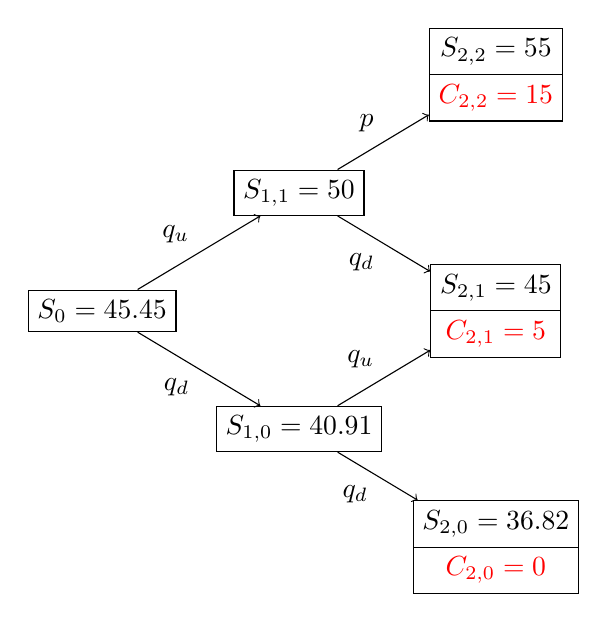
\begin{tikzpicture}[level distance=2.5cm]
    \tikzstyle{level 0}=[rectangle, draw]
    \tikzstyle{level 1}=[rectangle, draw]
    \tikzstyle{level 2}=[rectangle split,rectangle split parts=2,draw]
    \tikzstyle{edge from parent}=[->,draw]
    \tikzstyle{blank}=[rectangle]
    \node[level 0] {$S_0 = 45.45$} [grow'=right,sibling distance=3cm]
      child {node[level 1] {$S_{1,1}=50$}
             child {node[level 2] {$S_{2,2}=55$\nodepart{second}\textcolor{red}{$C_{2,2}=15$}}
             edge from parent node[blank,above left] {$p$}
                   }
             child {node[level 2] {\phantom{$S_{2,1}=45$}\nodepart{second}\textcolor{red}{\phantom{$C_{2,1}=5$}}}
                    edge from parent node[blank,below left] {$q_d$}
                   }
             edge from parent node[blank,above left] {$q_u$}
            }
      child {node[level 1] {$S_{1,0}=40.91$}
             child {node[level 2] {$S_{2,1}=45$\nodepart{second}\textcolor{red}{$C_{2,1}=5$}}
                    edge from parent node[blank,above left] {$q_u$}
                   }
             child {node[level 2] {$S_{2,0}=36.82$\nodepart{second}\textcolor{red}{$C_{2,0}=0$}}
                    edge from parent node[blank,below left] {$q_d$}
                   }
             edge from parent node[blank,below left] {$q_d$}
            };
\end{tikzpicture}

The risk-neutral probabilities are identical at all nodes:

\[\begin{aligned}
    q_u &=& \frac{\rho-d}{u-d} = \frac{1.05-.9}{1.1-.9} = .75  \\
    q_d &=& .25\end{aligned}\]

Using these values, the option value one step prior to expiry can be
computed using (\[eq:cox-ross-1\]):

\[\begin{aligned}
C_{1,1} &=& \frac{1}{\rho}(q_u C_{2,2} + q_d C_{2,1}) = 11.90  \\
C_{1,0} &=& \frac{1}{\rho}(q_u C_{2,1} + q_d C_{2,0}) = 3.57 \\\end{aligned}\]

The reasoning that led to (\[eq:cox-ross-1\]) applies however to any
node, and in particular to node (0,0). The option price at that node is
thus:

\[C_{0,0} = \frac{1}{\rho}(q_u C_{1,1} + q_d C_{1,0}) = 9.35\]

The process is pictured in Figure~\[fig:bin-tree-3\].

\hypertarget{american-exercise}{%
\section{American Exercise}\label{american-exercise}}

American exercise refer to the right to exercise the option at any time
before expiry. Clearly, an option with American exercise is worth more
than the comparable option with European exercise. To price an American
option, we introduce the notion of continuation value. The continuation
value \(V^i_t\) at node \(i\) and time \(t\) is the option value, assuming
that it will be exercised after time \(t\). At each step, one determines
the optimal decision by comparing the value of an immediate exercise to
the continuation value. The option value is therefore, for a call:

\[\begin{aligned}
C^i_t  &=& \max(S^i_t - K, V^i_t) \\
       &=& \max(S^i_t-K, \frac{1}{\rho} (q_u C^{i+1}_{t+1} + q_d C^{i}_{t+1}))
     \end{aligned}\]

Starting from the data of the previous section, we now assume that the
stock pays a dividend of 3 €~in period 2. The modified tree is
represented in figure~\[fig:bin-tree-4\].

We price an American call struck at 40€~in this tree. Exercise values in
period 2 are computed as before, giving the following values:

\[\begin{aligned}
C_{2,2} &=& 12 \\
C_{2,1} &=& 0 \\
C_{2,0} &=& 0 \end{aligned}\]

At period 1, the option holder determines the optimal policy: exercise
immediately or hold the option until period 2. The resulting values are:

\[\begin{aligned}
C_{1,1} &=& \max((50-40), \frac{1}{\rho} (q_u 10 + q_d 2)) = 10 \\
C_{1,0} &=& \max((40.91-40), \frac{1}{\rho} (q_u 2 + q_d 0)) = 1.42 \\\end{aligned}\]

The option value today is finally determined to be:

\[\begin{aligned}
C_{0,0} &=& \max(5.45, \frac{1}{\rho} (q_u 10  + q_d 1.42)) \\
&=& 7.48\end{aligned}\]

Under the same conditions, a European option is worth \(C_{0,0} = 6.79\).
The difference comes from the early exercise of the American option in
node (1,1).

\hypertarget{calibration-of-the-binomial-model}{%
\section{Calibration of the Binomial Model}\label{calibration-of-the-binomial-model}}

With interest rate assumed to be known, option prices are determined by
the terms \(u\) and \(d\) that describe the binomial branching process. How
should \(u\) and \(d\) be chosen?

The time interval \([0, T]\) is divided into \(N\) equal steps
\([t_j , t_{j+1}]\) of length \(\Delta t\). Assume that the process for the
underlying asset \(S_t\) is such that \(V_t = \ln(S_t/S_{t-\Delta t})\) are
iid random variables with mean \(\mu \Delta t\) and variance
\(\sigma^2 \Delta t\).

\[S_{t_j} = S_{t_{j-1}} e^{V_j}\]

Let's determine \(u\) and \(d\) by matching the mean and variance of \(V_t\)
and of the binomial process:

\[\begin{aligned}
E(V_j) & = & p \ln u + (1-p) \ln d \\
& = & \mu \Delta t \\
V(V_j) & = & E(V_j^2) - E(V_j)^2 \\
& = & \sigma^2 \Delta t\end{aligned}\]

Which forms a system of 2 equations and three unknown. Without loss of
generality, set \(p=1/2\), to obtain:

\[\begin{aligned}
\frac{1}{2} (\ln u + \ln d) &=& \mu \Delta t \\
\frac{1}{4} (\ln u + \ln d)^2 &=& \sigma^2 \Delta t\end{aligned}\]

The solution is:

\[\begin{aligned}
u &=& e^{\mu \Delta t + \sigma \sqrt{\Delta t}} \nonumber \\
d &=& e^{\mu \Delta t - \sigma \sqrt{\Delta t}}
\label{eq:ud}\end{aligned}\]

The corresponding value of the risk-neutral up probability, \(q_u\) is

\[q_u = \frac{e^{r\Delta t} - e^{\mu \Delta t - \sigma \sqrt{\Delta t}}}{e^{\mu \Delta t + \sigma \sqrt{\Delta t}} - e^{\mu \Delta t - \sigma \sqrt{\Delta t}}}
\label{eq:qu}\]

This is the single-period risk-neutral probability, not the objective
probability \(p\). We next compute the limit of \(q_u\) as
\(\Delta t \rightarrow 0\).

We use the following first order approximation:

\[\begin{aligned}
    e^{\mu \Delta t + \sigma \sqrt{\Delta t}} &=& (1+\mu \Delta t + \sigma \sqrt{\Delta t} + \frac{1}{2}(\mu \Delta t + \sigma \sqrt{\Delta t})^2 + \ldots \\
    &=& 1+\mu \Delta t + \sigma \sqrt{\Delta t} +
    \frac{1}{2} \sigma^2 \Delta t + O(\Delta t^{3/2})\end{aligned}\]

and similarly,

\[e^{\mu \Delta t - \sigma \sqrt{\Delta t}} =
    1+\mu \Delta t - \sigma \sqrt{\Delta t} + \frac{1}{2} \sigma^2 \Delta t + O(\Delta t^{3/2})\]

Combining these approximations with (\[eq:qu\]) yields,

\[\begin{aligned}
q_u &=& \frac{\sigma \sqrt{\Delta t} + (r-\frac{1}{2} \sigma^2 - \mu) \Delta t + O(\Delta t ^{3/2})}{2 \sigma \sqrt{\Delta t} + O(\Delta t ^{3/2})}  \nonumber \\
&=& \frac{1}{2} + \frac{r-\frac{1}{2} \sigma^2 - \mu}{2 \sigma} \sqrt{\Delta t}  + O(\Delta t)
\label{eq:qu-2}\end{aligned}\]

Let's now use these expressions for \(q_u\) to compute the mean and
variance of \(V_j\).

\[E(V_j) = q_u \ln u + (1-q_u) \ln d\]

Use (\[eq:ud\]) to get:

\[E(V_j) = q_u (2\sigma\sqrt{\Delta t}) + \mu \Delta t - \sigma \sqrt{\Delta t}\]

Substitute \(q_u\) by its value (\[eq:qu\]) to get:

\[E(V_j) = (r-\frac{1}{2} \sigma^2) \Delta t + O(\Delta t ^{3/2})\]

Similarly,

\[Var(V_j) = \sigma^2 \Delta t + O(\Delta t^{3/2})\]

The remarkable point of this result is that \(\mu\) no longer appears.

Extending the reasoning of Section~\[subsec:binomial\] to multiple
periods, we write that under the risk neutral probability \(q_u, q_d\),
the option value is the discounted expected value of the payoff:

\[\begin{aligned}
P(S_0) &=& e^{-rT} E^Q(f(S_T)) \\
 &=& e^{-rT} E^Q(f(S_0e^{\sum_{i=1}^N V_i})) \nonumber
\label{eq:pso}\end{aligned}\]

where \(f(S_T)\) is the payoff at expiry. We next need to compute the
limit: \[\lim_{N\to\infty} \sum_{i=1}^N V_i\]

The variables \(V_i\) are a function of \(N\), thus the Central Limit
Theorem cannot be used as such. However, we can invoke Lindeberg's
condition to obtain the same result:

\emph{(Lindeberg's Condition)} Let \(X_k, k \in N\) be independent variables
with \(E(X_k)=\mu_k\) and \(V(X_k) = \sigma^2_k\). Let
\(s_n^2 = \sum_i^n \sigma^2_i\). If the variables satisfy Lindeberg's
condition, then
\[Z_n = \frac{\sum_{k=1}^n (X_k - \mu_k)}{s_n} \rightarrow N(0, 1)\]

To simplify notation, let \(E^Q(V_i) = a\), \(Var^Q(V_i) = b\), Lindeberg's
condition yields:

\[\frac{\sum_i^N V_i - Na }{b \sqrt{N}} \rightarrow N(0,1)\]

\[\frac{\sum_i^N V_i - Na }{b \sqrt{N}} = \frac{\sum_i^N V_i - (r-\frac{1}{2} \sigma^2)T + O(N^{-1/2}) }{\sigma \sqrt{T} + O(N^{-1/2})}\]

\[\frac{\sum_i^N V_i - (r-\frac{1}{2} \sigma^2)T}{\sigma \sqrt{T})} \rightarrow N(0,1)\]

Thus,

\[\sum_i^N V_i \rightarrow  N \left( (r-\frac{1}{2} \sigma^2)T, \sigma^2 T \right)\]

Finally, as \(N \rightarrow \infty\), (\[eq:pso\]) becomes:

\[P(S_0) = \frac{e^{-rT}}{\sqrt{2\pi}} \int_{-\infty}^{\infty} f(S_0e^{(r-\frac{1}{2} \sigma^2)T + \sigma \sqrt{T}} e^{-\frac{1}{2} u^2} du\]

which is the Black-Scholes valuation formula, as derived by
Cox, Ross, and Rubinstein (\protect\hyperlink{ref-JohnC.Cox1979}{1979}). Again, the significance of this result is that \(\mu\)
does not appear in the formula.

\hypertarget{tree-geometry}{%
\subsection{Tree Geometry}\label{tree-geometry}}

We now use the result from the previous section to determine the
geometry of the tree and the risk-neutral transition probabilities,
consistent with the parameters of the diffusion process.

Recall from the previous section that \(u\) and \(d\) are defined by:

\[\begin{aligned}
u &=& e^{\mu \Delta t + \sigma \sqrt{\Delta t}} \\
d &=& e^{\mu \Delta t - \sigma \sqrt{\Delta t}}\end{aligned}\]

Ultimately, \(\mu\) does not appear in the valuation formula, it can thus
be set to an arbitrary value without loss of generality.

In the original CRR model, \(\mu = 0\), which leads to:

\[\begin{aligned}
 u &=& e^{\sigma \sqrt{t}} \\
d &=& e^{-\sigma \sqrt{t}} \\
q_u &=& \frac{e^{rt} - e^{-\sigma \sqrt{t}}}{e^{\sigma \sqrt{t}} - e^{-\sigma \sqrt{t}}}\end{aligned}\]

There are many other possibilities: a popular choice introduced by
Jarrow and Rudd (\protect\hyperlink{ref-R.Jarrow1993}{1993}) is to set \(\mu\) so that transition probabilities are equal
to \(\frac{1}{2}\). Using (\[eq:qu-2\]), this involves setting
\(\mu=r-\frac{1}{2}\sigma^2\), and the branching process is then:
\[\begin{aligned}
 u &=& e^{(r-\frac{1}{2} \sigma^2)\Delta t + \sigma \sqrt{\Delta t}} \\
d &=& e^{(r-\frac{1}{2} \sigma^2)\Delta t -\sigma \sqrt{\Delta t}} \\
q_u &=& \frac{1}{2}\end{aligned}\]

There are many other possible choices, but no significant differences in
the convergence rate to the Black-Scholes option value. Most of the
models, however, suffer from a form of instability which is now
described.

\hypertarget{stability-of-the-binomial-model}{%
\chapter{Stability of the Binomial Model}\label{stability-of-the-binomial-model}}

\texttt{\{r\ tufte::newthought("We")\}} would like to verify the convergence of the Cox-Ross model to the
Black-Scholes price as the number of steps \(N\) increases. This can be
investigated with the following script:

\begin{Shaded}
\begin{Highlighting}[]
\NormalTok{Strike \textless{}{-}}\StringTok{ }\DecValTok{100}
\NormalTok{Spot \textless{}{-}}\StringTok{ }\DecValTok{100}
\NormalTok{T1 \textless{}{-}}\StringTok{ }\DecValTok{1}\OperatorTok{/}\DecValTok{4}
\NormalTok{r \textless{}{-}}\StringTok{ }\FloatTok{0.05}
\NormalTok{b \textless{}{-}}\StringTok{ }\FloatTok{0.05}
\NormalTok{sigma \textless{}{-}}\StringTok{ }\FloatTok{0.3}

\NormalTok{NN \textless{}{-}}\StringTok{ }\KeywordTok{seq}\NormalTok{(}\DecValTok{20}\NormalTok{, }\DecValTok{100}\NormalTok{, }\DecValTok{1}\NormalTok{)}
\NormalTok{nb \textless{}{-}}\StringTok{ }\KeywordTok{length}\NormalTok{(NN)}
\NormalTok{res \textless{}{-}}\StringTok{ }\KeywordTok{matrix}\NormalTok{(}\DataTypeTok{nrow =}\NormalTok{ nb, }\DataTypeTok{ncol =} \DecValTok{2}\NormalTok{)}
\NormalTok{bs \textless{}{-}}\StringTok{ }\KeywordTok{rep}\NormalTok{(}\DecValTok{0}\NormalTok{, }\DecValTok{2}\NormalTok{)}

\CommentTok{\# The Black{-}Scholes price}
\NormalTok{bs[}\DecValTok{1}\NormalTok{] \textless{}{-}}\StringTok{ }\KeywordTok{GBSOption}\NormalTok{(}\DataTypeTok{TypeFlag =} \StringTok{"c"}\NormalTok{, }\DataTypeTok{S =}\NormalTok{ Spot, }\DataTypeTok{X =}\NormalTok{ Strike,}
    \DataTypeTok{Time =}\NormalTok{ T1, }\DataTypeTok{r =}\NormalTok{ r, }\DataTypeTok{b =}\NormalTok{ b, }\DataTypeTok{sigma =}\NormalTok{ sigma)}\OperatorTok{@}\NormalTok{price}
\NormalTok{bs[}\DecValTok{2}\NormalTok{] \textless{}{-}}\StringTok{ }\KeywordTok{GBSOption}\NormalTok{(}\DataTypeTok{TypeFlag =} \StringTok{"c"}\NormalTok{, }\DataTypeTok{S =}\NormalTok{ Spot, }\DataTypeTok{X =}\NormalTok{ Strike }\OperatorTok{+}
\StringTok{    }\DecValTok{10}\NormalTok{, }\DataTypeTok{Time =}\NormalTok{ T1, }\DataTypeTok{r =}\NormalTok{ r, }\DataTypeTok{b =}\NormalTok{ b, }\DataTypeTok{sigma =}\NormalTok{ sigma)}\OperatorTok{@}\NormalTok{price}

\CommentTok{\# Binomial price, function of number of}
\CommentTok{\# steps}
\NormalTok{res[, }\DecValTok{1}\NormalTok{] \textless{}{-}}\StringTok{ }\KeywordTok{sapply}\NormalTok{(NN, }\ControlFlowTok{function}\NormalTok{(n) }\KeywordTok{CRRBinomialTreeOption}\NormalTok{(}\DataTypeTok{TypeFlag =} \StringTok{"ce"}\NormalTok{,}
    \DataTypeTok{S =}\NormalTok{ Spot, }\DataTypeTok{X =}\NormalTok{ Strike, }\DataTypeTok{Time =}\NormalTok{ T1, }\DataTypeTok{r =}\NormalTok{ r, }\DataTypeTok{b =}\NormalTok{ b,}
    \DataTypeTok{sigma =}\NormalTok{ sigma, n)}\OperatorTok{@}\NormalTok{price)}

\NormalTok{res[, }\DecValTok{2}\NormalTok{] \textless{}{-}}\StringTok{ }\KeywordTok{sapply}\NormalTok{(NN, }\ControlFlowTok{function}\NormalTok{(n) }\KeywordTok{CRRBinomialTreeOption}\NormalTok{(}\DataTypeTok{TypeFlag =} \StringTok{"ce"}\NormalTok{,}
    \DataTypeTok{S =}\NormalTok{ Spot, }\DataTypeTok{X =}\NormalTok{ Strike }\OperatorTok{+}\StringTok{ }\DecValTok{10}\NormalTok{, }\DataTypeTok{Time =}\NormalTok{ T1, }\DataTypeTok{r =}\NormalTok{ r,}
    \DataTypeTok{b =}\NormalTok{ b, }\DataTypeTok{sigma =}\NormalTok{ sigma, n)}\OperatorTok{@}\NormalTok{price)}
\end{Highlighting}
\end{Shaded}

A plot of the prices as a function of the number of steps
(Figure~\[fig:bin-conv\]) shows an oscillating pattern:

\begin{Shaded}
\begin{Highlighting}[]
\KeywordTok{par}\NormalTok{(}\DataTypeTok{mfrow =} \KeywordTok{c}\NormalTok{(}\DecValTok{1}\NormalTok{, }\DecValTok{2}\NormalTok{))}
\KeywordTok{plot}\NormalTok{(NN, res[, }\DecValTok{1}\NormalTok{], }\DataTypeTok{type =} \StringTok{"l"}\NormalTok{, }\DataTypeTok{main =} \StringTok{"ATM"}\NormalTok{, }\DataTypeTok{xlab =} \StringTok{"Number of steps"}\NormalTok{,}
    \DataTypeTok{ylab =} \StringTok{"price"}\NormalTok{, }\DataTypeTok{col =} \StringTok{"blue"}\NormalTok{, }\DataTypeTok{ylim =} \KeywordTok{c}\NormalTok{(}\KeywordTok{min}\NormalTok{(res[,}
        \DecValTok{1}\NormalTok{]), }\KeywordTok{max}\NormalTok{(res[, }\DecValTok{1}\NormalTok{])))}
\KeywordTok{abline}\NormalTok{(}\DataTypeTok{h =}\NormalTok{ bs[}\DecValTok{1}\NormalTok{], }\DataTypeTok{lwd =} \DecValTok{2}\NormalTok{, }\DataTypeTok{col =} \StringTok{"red"}\NormalTok{)}

\KeywordTok{plot}\NormalTok{(NN, res[, }\DecValTok{2}\NormalTok{], }\DataTypeTok{type =} \StringTok{"l"}\NormalTok{, }\DataTypeTok{main =} \StringTok{"OTM"}\NormalTok{, }\DataTypeTok{xlab =} \StringTok{"Number of steps"}\NormalTok{,}
    \DataTypeTok{ylab =} \StringTok{"price"}\NormalTok{, }\DataTypeTok{col =} \StringTok{"blue"}\NormalTok{, }\DataTypeTok{ylim =} \KeywordTok{c}\NormalTok{(}\KeywordTok{min}\NormalTok{(res[,}
        \DecValTok{2}\NormalTok{]), }\KeywordTok{max}\NormalTok{(res[, }\DecValTok{2}\NormalTok{])))}
\KeywordTok{abline}\NormalTok{(}\DataTypeTok{h =}\NormalTok{ bs[}\DecValTok{2}\NormalTok{], }\DataTypeTok{lwd =} \DecValTok{2}\NormalTok{, }\DataTypeTok{col =} \StringTok{"red"}\NormalTok{)}
\KeywordTok{par}\NormalTok{(}\DataTypeTok{mfrow =} \KeywordTok{c}\NormalTok{(}\DecValTok{1}\NormalTok{, }\DecValTok{1}\NormalTok{))}
\end{Highlighting}
\end{Shaded}

\includegraphics{203-Binomial2_files/figure-latex/fig-bin-conv-a-1}

Other binomial algorithms, such as Tian's, exhibit a similar pattern, as
evidenced in Figure~\[fig:bin-conv-2\]. The horizontal line marks the
Black-Scholes price.

\includegraphics{203-Binomial2_files/figure-latex/fig-bin-conv-2-a-1}

This sawtooth pattern is due to the position of the strike relative to
the sequence of nodes at expiry;
we describe below some computational strategies
for smoothing these oscillations and speeding up the convergence of
binomial trees. See
Joshi (\protect\hyperlink{ref-Joshi2007}{2007}) for an extensive survey of binomial models with
improved convergence properties.

Since the oscillations are caused by the variations in the relative
position of the strike with respect to nodes at expiry, a natural
strategy, introduced by Leisen and Reimer (\protect\hyperlink{ref-Leisen1996}{1996}), is to construct the tree such that
the strike coincides with a node. This is achieved by setting
\[\mu = \frac{1}{T} \log \left(\frac{K}{S_0} \right)\]

The resulting tree is centered on \(K\) in log space. The pricing method
is implemented as follows:

\begin{Shaded}
\begin{Highlighting}[]
\NormalTok{CRRWithDrift \textless{}{-}}\StringTok{ }\ControlFlowTok{function}\NormalTok{(}\DataTypeTok{TypeFlag =} \KeywordTok{c}\NormalTok{(}\StringTok{"ce"}\NormalTok{, }\StringTok{"pe"}\NormalTok{,}
    \StringTok{"ca"}\NormalTok{, }\StringTok{"pa"}\NormalTok{), S, X, Time, r, mu, sigma, n) \{}
\NormalTok{    TypeFlag =}\StringTok{ }\NormalTok{TypeFlag[}\DecValTok{1}\NormalTok{]}
\NormalTok{    z =}\StringTok{ }\OtherTok{NA}
    \ControlFlowTok{if}\NormalTok{ (TypeFlag }\OperatorTok{==}\StringTok{ "ce"} \OperatorTok{||}\StringTok{ }\NormalTok{TypeFlag }\OperatorTok{==}\StringTok{ "ca"}\NormalTok{)}
\NormalTok{        z =}\StringTok{ }\OperatorTok{+}\DecValTok{1}
    \ControlFlowTok{if}\NormalTok{ (TypeFlag }\OperatorTok{==}\StringTok{ "pe"} \OperatorTok{||}\StringTok{ }\NormalTok{TypeFlag }\OperatorTok{==}\StringTok{ "pa"}\NormalTok{)}
\NormalTok{        z =}\StringTok{ }\DecValTok{{-}1}
    \ControlFlowTok{if}\NormalTok{ (}\KeywordTok{is.na}\NormalTok{(z))}
        \KeywordTok{stop}\NormalTok{(}\StringTok{"TypeFlag misspecified: ce|ca|pe|pa"}\NormalTok{)}
\NormalTok{    dt =}\StringTok{ }\NormalTok{Time}\OperatorTok{/}\NormalTok{n}
\NormalTok{    u =}\StringTok{ }\KeywordTok{exp}\NormalTok{(mu }\OperatorTok{*}\StringTok{ }\NormalTok{dt }\OperatorTok{+}\StringTok{ }\NormalTok{sigma }\OperatorTok{*}\StringTok{ }\KeywordTok{sqrt}\NormalTok{(dt))}
\NormalTok{    d =}\StringTok{ }\KeywordTok{exp}\NormalTok{(mu }\OperatorTok{*}\StringTok{ }\NormalTok{dt }\OperatorTok{{-}}\StringTok{ }\NormalTok{sigma }\OperatorTok{*}\StringTok{ }\KeywordTok{sqrt}\NormalTok{(dt))}

\NormalTok{    p =}\StringTok{ }\NormalTok{(}\KeywordTok{exp}\NormalTok{(r }\OperatorTok{*}\StringTok{ }\NormalTok{dt) }\OperatorTok{{-}}\StringTok{ }\NormalTok{d)}\OperatorTok{/}\NormalTok{(u }\OperatorTok{{-}}\StringTok{ }\NormalTok{d)}
\NormalTok{    Df =}\StringTok{ }\KeywordTok{exp}\NormalTok{(}\OperatorTok{{-}}\NormalTok{r }\OperatorTok{*}\StringTok{ }\NormalTok{dt)}

    \CommentTok{\# underlying asset at step N{-}1}
\NormalTok{    ST \textless{}{-}}\StringTok{ }\NormalTok{S }\OperatorTok{*}\StringTok{ }\NormalTok{(d}\OperatorTok{\^{}}\NormalTok{(n }\OperatorTok{{-}}\StringTok{ }\DecValTok{1}\NormalTok{)) }\OperatorTok{*}\StringTok{ }\KeywordTok{cumprod}\NormalTok{(}\KeywordTok{c}\NormalTok{(}\DecValTok{1}\NormalTok{, }\KeywordTok{rep}\NormalTok{((u}\OperatorTok{/}\NormalTok{d),}
\NormalTok{        n }\OperatorTok{{-}}\StringTok{ }\DecValTok{1}\NormalTok{)))}
    \CommentTok{\# at step (n{-}1), value an European}
    \CommentTok{\# option of maturity dt}
\NormalTok{    BSTypeFlag \textless{}{-}}\StringTok{ }\KeywordTok{substr}\NormalTok{(TypeFlag, }\DecValTok{1}\NormalTok{, }\DecValTok{1}\NormalTok{)}
\NormalTok{    OptionValue \textless{}{-}}\StringTok{ }\KeywordTok{GBSOption}\NormalTok{(BSTypeFlag, ST, X,}
\NormalTok{        dt, r, b, sigma)}\OperatorTok{@}\NormalTok{price}

    \ControlFlowTok{if}\NormalTok{ (TypeFlag }\OperatorTok{==}\StringTok{ "ce"} \OperatorTok{||}\StringTok{ }\NormalTok{TypeFlag }\OperatorTok{==}\StringTok{ "pe"}\NormalTok{) \{}
        \ControlFlowTok{for}\NormalTok{ (j }\ControlFlowTok{in} \KeywordTok{seq}\NormalTok{(}\DataTypeTok{from =}\NormalTok{ n }\OperatorTok{{-}}\StringTok{ }\DecValTok{2}\NormalTok{, }\DataTypeTok{to =} \DecValTok{0}\NormalTok{, }\DataTypeTok{by =} \DecValTok{{-}1}\NormalTok{)) OptionValue \textless{}{-}}\StringTok{ }\NormalTok{(p }\OperatorTok{*}
\StringTok{            }\NormalTok{OptionValue[}\DecValTok{2}\OperatorTok{:}\NormalTok{(j }\OperatorTok{+}\StringTok{ }\DecValTok{2}\NormalTok{)] }\OperatorTok{+}\StringTok{ }\NormalTok{(}\DecValTok{1} \OperatorTok{{-}}\StringTok{ }\NormalTok{p) }\OperatorTok{*}
\StringTok{            }\NormalTok{OptionValue[}\DecValTok{1}\OperatorTok{:}\NormalTok{(j }\OperatorTok{+}\StringTok{ }\DecValTok{1}\NormalTok{)]) }\OperatorTok{*}\StringTok{ }\NormalTok{Df}
\NormalTok{    \}}

    \ControlFlowTok{if}\NormalTok{ (TypeFlag }\OperatorTok{==}\StringTok{ "ca"} \OperatorTok{||}\StringTok{ }\NormalTok{TypeFlag }\OperatorTok{==}\StringTok{ "pa"}\NormalTok{) \{}
        \ControlFlowTok{for}\NormalTok{ (j }\ControlFlowTok{in} \KeywordTok{seq}\NormalTok{(}\DataTypeTok{from =}\NormalTok{ n }\OperatorTok{{-}}\StringTok{ }\DecValTok{2}\NormalTok{, }\DataTypeTok{to =} \DecValTok{0}\NormalTok{, }\DataTypeTok{by =} \DecValTok{{-}1}\NormalTok{)) \{}
\NormalTok{            ContValue \textless{}{-}}\StringTok{ }\NormalTok{(p }\OperatorTok{*}\StringTok{ }\NormalTok{OptionValue[}\DecValTok{2}\OperatorTok{:}\NormalTok{(j }\OperatorTok{+}
\StringTok{                }\DecValTok{2}\NormalTok{)] }\OperatorTok{+}\StringTok{ }\NormalTok{(}\DecValTok{1} \OperatorTok{{-}}\StringTok{ }\NormalTok{p) }\OperatorTok{*}\StringTok{ }\NormalTok{OptionValue[}\DecValTok{1}\OperatorTok{:}\NormalTok{(j }\OperatorTok{+}
\StringTok{                }\DecValTok{1}\NormalTok{)]) }\OperatorTok{*}\StringTok{ }\NormalTok{Df}
\NormalTok{            ST \textless{}{-}}\StringTok{ }\NormalTok{S }\OperatorTok{*}\StringTok{ }\NormalTok{(d}\OperatorTok{\^{}}\NormalTok{j) }\OperatorTok{*}\StringTok{ }\KeywordTok{cumprod}\NormalTok{(}\KeywordTok{c}\NormalTok{(}\DecValTok{1}\NormalTok{, }\KeywordTok{rep}\NormalTok{((u}\OperatorTok{/}\NormalTok{d),}
\NormalTok{                j)))}
\NormalTok{            OptionValue \textless{}{-}}\StringTok{ }\KeywordTok{sapply}\NormalTok{(}\DecValTok{1}\OperatorTok{:}\NormalTok{(j }\OperatorTok{+}\StringTok{ }\DecValTok{1}\NormalTok{), }\ControlFlowTok{function}\NormalTok{(i) }\KeywordTok{max}\NormalTok{(ST[i] }\OperatorTok{{-}}
\StringTok{                }\NormalTok{X, ContValue[i]))}
\NormalTok{        \}}
\NormalTok{    \}}

\NormalTok{    OptionValue[}\DecValTok{1}\NormalTok{]}
\NormalTok{\}}
\end{Highlighting}
\end{Shaded}

Convergence of the model as \(N\) increases is significantly improved, as
evidenced by the graphs in Figure~\[fig:CRRWithDrift\].

\includegraphics{203-Binomial2_files/figure-latex/fig-crrwithdrift-1}

In the context of an American option, note that if the option has not
been exercised at step \(N-1\), the option is now European, and can be
priced at these nodes with the Black-Scholes model, rather than with the
backward recursion from step \(N\) (the expiry date). This simple
modification smooths the option value at step \(N-1\) and cancels the
oscillations, as illustrated in figure~\[fig:bin-conv-crr-bs\], but at
the price of a substantial increase in computation time.

\begin{Shaded}
\begin{Highlighting}[]
\NormalTok{CRRWithBS \textless{}{-}}\StringTok{ }\ControlFlowTok{function}\NormalTok{(}\DataTypeTok{TypeFlag =} \KeywordTok{c}\NormalTok{(}\StringTok{"ce"}\NormalTok{, }\StringTok{"pe"}\NormalTok{,}
    \StringTok{"ca"}\NormalTok{, }\StringTok{"pa"}\NormalTok{), S, X, Time, r, b, sigma, n) \{}
\NormalTok{    TypeFlag =}\StringTok{ }\NormalTok{TypeFlag[}\DecValTok{1}\NormalTok{]}
\NormalTok{    z =}\StringTok{ }\OtherTok{NA}
    \ControlFlowTok{if}\NormalTok{ (TypeFlag }\OperatorTok{==}\StringTok{ "ce"} \OperatorTok{||}\StringTok{ }\NormalTok{TypeFlag }\OperatorTok{==}\StringTok{ "ca"}\NormalTok{)}
\NormalTok{        z =}\StringTok{ }\OperatorTok{+}\DecValTok{1}
    \ControlFlowTok{if}\NormalTok{ (TypeFlag }\OperatorTok{==}\StringTok{ "pe"} \OperatorTok{||}\StringTok{ }\NormalTok{TypeFlag }\OperatorTok{==}\StringTok{ "pa"}\NormalTok{)}
\NormalTok{        z =}\StringTok{ }\DecValTok{{-}1}
    \ControlFlowTok{if}\NormalTok{ (}\KeywordTok{is.na}\NormalTok{(z))}
        \KeywordTok{stop}\NormalTok{(}\StringTok{"TypeFlag misspecified: ce|ca|pe|pa"}\NormalTok{)}
\NormalTok{    dt =}\StringTok{ }\NormalTok{Time}\OperatorTok{/}\NormalTok{n}
\NormalTok{    u =}\StringTok{ }\KeywordTok{exp}\NormalTok{(sigma }\OperatorTok{*}\StringTok{ }\KeywordTok{sqrt}\NormalTok{(dt))}
\NormalTok{    d =}\StringTok{ }\DecValTok{1}\OperatorTok{/}\NormalTok{u}
\NormalTok{    p =}\StringTok{ }\NormalTok{(}\KeywordTok{exp}\NormalTok{(b }\OperatorTok{*}\StringTok{ }\NormalTok{dt) }\OperatorTok{{-}}\StringTok{ }\NormalTok{d)}\OperatorTok{/}\NormalTok{(u }\OperatorTok{{-}}\StringTok{ }\NormalTok{d)}
\NormalTok{    Df =}\StringTok{ }\KeywordTok{exp}\NormalTok{(}\OperatorTok{{-}}\NormalTok{r }\OperatorTok{*}\StringTok{ }\NormalTok{dt)}

    \CommentTok{\# underlying asset at step N{-}1}
\NormalTok{    ST \textless{}{-}}\StringTok{ }\NormalTok{S }\OperatorTok{*}\StringTok{ }\NormalTok{(d}\OperatorTok{\^{}}\NormalTok{(n }\OperatorTok{{-}}\StringTok{ }\DecValTok{1}\NormalTok{)) }\OperatorTok{*}\StringTok{ }\KeywordTok{cumprod}\NormalTok{(}\KeywordTok{c}\NormalTok{(}\DecValTok{1}\NormalTok{, }\KeywordTok{rep}\NormalTok{((u}\OperatorTok{/}\NormalTok{d),}
\NormalTok{        n }\OperatorTok{{-}}\StringTok{ }\DecValTok{1}\NormalTok{)))}
    \CommentTok{\# at step (n{-}1), value an European}
    \CommentTok{\# option of maturity dt}
\NormalTok{    BSTypeFlag \textless{}{-}}\StringTok{ }\KeywordTok{substr}\NormalTok{(TypeFlag, }\DecValTok{1}\NormalTok{, }\DecValTok{1}\NormalTok{)}
\NormalTok{    OptionValue \textless{}{-}}\StringTok{ }\KeywordTok{GBSOption}\NormalTok{(BSTypeFlag, ST, X,}
\NormalTok{        dt, r, b, sigma)}\OperatorTok{@}\NormalTok{price}

    \ControlFlowTok{if}\NormalTok{ (TypeFlag }\OperatorTok{==}\StringTok{ "ce"} \OperatorTok{||}\StringTok{ }\NormalTok{TypeFlag }\OperatorTok{==}\StringTok{ "pe"}\NormalTok{) \{}
        \ControlFlowTok{for}\NormalTok{ (j }\ControlFlowTok{in} \KeywordTok{seq}\NormalTok{(}\DataTypeTok{from =}\NormalTok{ n }\OperatorTok{{-}}\StringTok{ }\DecValTok{2}\NormalTok{, }\DataTypeTok{to =} \DecValTok{0}\NormalTok{, }\DataTypeTok{by =} \DecValTok{{-}1}\NormalTok{)) OptionValue \textless{}{-}}\StringTok{ }\NormalTok{(p }\OperatorTok{*}
\StringTok{            }\NormalTok{OptionValue[}\DecValTok{2}\OperatorTok{:}\NormalTok{(j }\OperatorTok{+}\StringTok{ }\DecValTok{2}\NormalTok{)] }\OperatorTok{+}\StringTok{ }\NormalTok{(}\DecValTok{1} \OperatorTok{{-}}\StringTok{ }\NormalTok{p) }\OperatorTok{*}
\StringTok{            }\NormalTok{OptionValue[}\DecValTok{1}\OperatorTok{:}\NormalTok{(j }\OperatorTok{+}\StringTok{ }\DecValTok{1}\NormalTok{)]) }\OperatorTok{*}\StringTok{ }\NormalTok{Df}
\NormalTok{    \}}

    \ControlFlowTok{if}\NormalTok{ (TypeFlag }\OperatorTok{==}\StringTok{ "ca"} \OperatorTok{||}\StringTok{ }\NormalTok{TypeFlag }\OperatorTok{==}\StringTok{ "pa"}\NormalTok{) \{}
        \ControlFlowTok{for}\NormalTok{ (j }\ControlFlowTok{in} \KeywordTok{seq}\NormalTok{(}\DataTypeTok{from =}\NormalTok{ n }\OperatorTok{{-}}\StringTok{ }\DecValTok{2}\NormalTok{, }\DataTypeTok{to =} \DecValTok{0}\NormalTok{, }\DataTypeTok{by =} \DecValTok{{-}1}\NormalTok{)) \{}
\NormalTok{            ContValue \textless{}{-}}\StringTok{ }\NormalTok{(p }\OperatorTok{*}\StringTok{ }\NormalTok{OptionValue[}\DecValTok{2}\OperatorTok{:}\NormalTok{(j }\OperatorTok{+}
\StringTok{                }\DecValTok{2}\NormalTok{)] }\OperatorTok{+}\StringTok{ }\NormalTok{(}\DecValTok{1} \OperatorTok{{-}}\StringTok{ }\NormalTok{p) }\OperatorTok{*}\StringTok{ }\NormalTok{OptionValue[}\DecValTok{1}\OperatorTok{:}\NormalTok{(j }\OperatorTok{+}
\StringTok{                }\DecValTok{1}\NormalTok{)]) }\OperatorTok{*}\StringTok{ }\NormalTok{Df}
\NormalTok{            ST \textless{}{-}}\StringTok{ }\NormalTok{S }\OperatorTok{*}\StringTok{ }\NormalTok{(d}\OperatorTok{\^{}}\NormalTok{j) }\OperatorTok{*}\StringTok{ }\KeywordTok{cumprod}\NormalTok{(}\KeywordTok{c}\NormalTok{(}\DecValTok{1}\NormalTok{, }\KeywordTok{rep}\NormalTok{((u}\OperatorTok{/}\NormalTok{d),}
\NormalTok{                j)))}
\NormalTok{            OptionValue \textless{}{-}}\StringTok{ }\KeywordTok{sapply}\NormalTok{(}\DecValTok{1}\OperatorTok{:}\NormalTok{(j }\OperatorTok{+}\StringTok{ }\DecValTok{1}\NormalTok{), }\ControlFlowTok{function}\NormalTok{(i) }\KeywordTok{max}\NormalTok{(ST[i] }\OperatorTok{{-}}
\StringTok{                }\NormalTok{X, ContValue[i]))}
\NormalTok{        \}}
\NormalTok{    \}}

\NormalTok{    OptionValue[}\DecValTok{1}\NormalTok{]}
\NormalTok{\}}
\end{Highlighting}
\end{Shaded}

\includegraphics{203-Binomial2_files/figure-latex/fig-CRRWithBS-1}

\hypertarget{sec:trinomial}{%
\chapter{Trinomial Models}\label{sec:trinomial}}

A natural extension of the binomial model is a trinomial model, that is,
a model with three possible future states at each time step and current
state.

\hypertarget{the-trinomial-tree}{%
\section{The Trinomial Tree}\label{the-trinomial-tree}}

The stock price at time \(t\) is \(S_t\). From \(t\) to \(t+\Delta t\), the
stock may move up to \(S_u\) with probability \(p_u\), down to \(S_d\) with
probability \(p_d\), or move to a middle state \(S_m\) with probability
\(1-p_u-p_d\). The probabilities and future states must satisfy the
following constraints:

\begin{enumerate}
\def\labelenumi{\arabic{enumi}.}
\item
  The expected value of the stock at \(t+\Delta t\) must be the forward
  price:
  \[p_u S_u + p_d S_d + (1-p_u-p_d) S_m = F = S e^{(r-\delta)\Delta t}\]
\item
  Variance:
  \[p_u (S_u-F)^2 + p_d(S_d-F)^2 +(1-p_u-p_d)(S_m-F)^2 = S^2\sigma^2\Delta t\]
\end{enumerate}

The first method for constructing trinomial trees is simply to combine
two steps of any binomial tree.

Recall that a CRR binomial tree is defined by:

\[\begin{aligned}
    u &=& e^{\sigma \sqrt{\Delta t}} \\
    d &=& e^{-\sigma \sqrt{\Delta t}} \\
    p &=& \frac{e^{rt} - e^{-\sigma \sqrt{\Delta t}}}{e^{\sigma \sqrt{\Delta t}} - e^{-\sigma \sqrt{\Delta t}}}\end{aligned}\]

Combining two steps at a time, we obtain a trinomial tree with

\[\begin{aligned}
    S_u &=& S e^{\sigma \sqrt{2 \Delta t}} \\
    S_m & = & S \\
    S_d &=& S e^{-\sigma \sqrt{2 \Delta t}} \\
    p_u &=& \left( \frac{e^{r \Delta t} - e^{-\sigma \sqrt{\Delta t}}}{e^{\sigma \sqrt{\Delta t}} - e^{-\sigma \sqrt{\Delta t}}} \right)^2 \\
    p_d &=& (1-\sqrt{p_u})^2\end{aligned}\]

To every binomial tree corresponds a trinomial tree, obtained by
aggregating two steps.

Another geometry can be defined by setting the middle node to
\(S\) (\textasciitilde{}\cite{Hull1997} p.~360):

\begin{eqnarray*}
    S_m &=& S  \\
    S_u &=& S_m e^{\sigma \sqrt{3 \Delta t}} \\
    S_d &=& S_m e^{-\sigma \sqrt{3 \Delta t}} \\
    p_u &=& -\sqrt{\frac{\Delta t}{12 \sigma^2}} \left(r-\frac{\sigma^2}{2} \right) + \frac{1}{6} \\
    p_d &=&  \sqrt{\frac{\Delta t}{12 \sigma^2}} \left(r-\frac{\sigma^2}{2} \right) + \frac{1}{6}
\end{eqnarray*}

\hypertarget{bibliography}{%
\chapter{Bibliography}\label{bibliography}}

\hypertarget{refs}{}
\begin{cslreferences}
\leavevmode\hypertarget{ref-JohnC.Cox1979}{}%
Cox, J C, Stephen A Ross, and Mark Rubinstein. 1979. ``Option pricing: a simplified approach.'' \emph{Journal of Financial Econometrics} 7: 229--63.

\leavevmode\hypertarget{ref-R.Jarrow1993}{}%
Jarrow, Robert, and Andrew Rudd. 1993. \emph{Option pricing}. Richard D. Irwin.

\leavevmode\hypertarget{ref-Joshi2007}{}%
Joshi, Mark S. 2007. ``The Convergence of Binomial Trees for Pricing the American Put.'' \url{ssrn.com/abstract=1030143}.

\leavevmode\hypertarget{ref-Leisen1996}{}%
Leisen, D P J, and M Reimer. 1996. ``Binomial Models for Option Valuation - Examining and Improving Convergence.'' \emph{Applied Mathematical Finance} 3: 319--46.
\end{cslreferences}


\printindex

\end{document}
